%\documentclass[times]{fldauth}
\documentclass[times,doublespace]{fldauth}%For paper submission

% \usepackage[dvips,colorlinks,bookmarksopen,bookmarksnumbered,citecolor=red,urlcolor=red]{hyperref}
\usepackage[colorlinks,bookmarksopen,bookmarksnumbered,citecolor=red,urlcolor=red]{hyperref}

\newcommand\BibTeX{{\rmfamily B\kern-.05em \textsc{i\kern-.025em b}\kern-.08em
T\kern-.1667em\lower.7ex\hbox{E}\kern-.125emX}}

\def\volumeyear{201?}


%%%%%%%%%%%%%%%%%%%%%%%
%%%%%%%%%%%%%%%%%%%%%%%
\usepackage{amsmath}
\usepackage{amsthm}
\usepackage{amsfonts}
\usepackage{amsfonts}
\usepackage{color}
\usepackage{setspace}
%\usepackage{listings}
%\lstset{language=C++}
%\usepackage{lscape} 
\usepackage{float}
\usepackage{graphicx}
\usepackage{caption}
\usepackage{subcaption}
\usepackage[titletoc,toc]{appendix}
\usepackage{xspace}
%\usepackage{color}
%\textwidth = 450pt
\def\fxnote#1{\marginpar{\textcolor{green}{#1}}}
\def\fxwarning#1{\marginpar{\textcolor{red}{#1}}}
%\usepackage[a4paper]{geometry}
%
%=================================================================================================
% new commands
% +++++++++++++++++++++++++++++++++++++++++++++++++++++++++++++++++++++++++++++++++++++++++++++++++
\newcommand{\nc}{\newcommand}

% operators
\renewcommand{\div}{\mbold{\nabla}\! \cdot \!}
\newcommand{\grad}{\mbold{\nabla}}
\newcommand{\divv}[1]{\boldsymbol{\nabla}^{#1}\! \cdot \!}
\newcommand{\gradd}[1]{\mbold{\nabla}^{#1}}
\newcommand{\mbold}[1]{\boldsymbol#1}
% latex shortcuts
\newcommand{\bea}{\begin{eqnarray}}
\newcommand{\eea}{\end{eqnarray}}
\newcommand{\be}{\begin{equation}}
\newcommand{\ee}{\end{equation}}
\newcommand{\bal}{\begin{align}}
\newcommand{\eali}{\end{align}}
\newcommand{\bi}{\begin{itemize}}
\newcommand{\ei}{\end{itemize}}
\newcommand{\ben}{\begin{enumerate}}
\newcommand{\een}{\end{enumerate}}
\usepackage{amsthm}
\newtheorem*{remark}{Remark}
% DGFEM commands
\newcommand{\jmp}[1]{[\![#1]\!]}                     % jump
\newcommand{\mvl}[1]{\{\!\!\{#1\}\!\!\}}             % mean value
\newcommand{\keff}{\ensuremath{k_{\textit{eff}}}\xspace}
% shortcut for domain notation
\newcommand{\D}{\mathcal{D}}
% vector shortcuts
\newcommand{\vo}{\mbold{\Omega}}
\newcommand{\vr}{\mbold{r}}
\newcommand{\vn}{\mbold{n}}
\newcommand{\vnk}{\mbold{\mathbf{n}}}
\newcommand{\vj}{\mbold{J}}
\newcommand{\eig}[1]{\| #1 \|_2}
%
\newcommand{\EI}{\mathcal{E}_h^i}
\newcommand{\ED}{\mathcal{E}_h^{\partial \D^d}}
\newcommand{\EN}{\mathcal{E}_h^{\partial \D^n}}
\newcommand{\ER}{\mathcal{E}_h^{\partial \D^r}}
\newcommand{\reg}{\textit{reg}}
%
\newcommand{\norm}{\textrm{norm}}
\renewcommand{\Re}{\textrm{Re}}
\newcommand{\Pe}{\textrm{P\'e}}
\renewcommand{\Pr}{\textrm{Pr}}
%
\newcommand{\resi}{R}
%\newcommand{\resinew}{\tilde{D}_e}
\newcommand{\resinew}{\widetilde{\resi}}
\newcommand{\resisource}{\widetilde{\resi}^{source}}
\newcommand{\matder}[1]{\frac{\textrm{D} #1}{\textrm{D} t}}
%
% extra space
\newcommand{\qq}{\quad\quad}
% common reference commands
\newcommand{\eqt}[1]{Eq.~(\ref{#1})}                     % equation
\newcommand{\fig}[1]{Fig.~\ref{#1}}                      % figure
\newcommand{\tbl}[1]{Table~\ref{#1}}                     % table
\newcommand{\sct}[1]{Section~\ref{#1}}                   % section
\newcommand{\app}[1]{Appendix~\ref{#1}}                   % appendix
%
\newcommand{\ie}{i.e.,\@\xspace}
\newcommand{\eg}{e.g.,\@\xspace}
\newcommand{\psc}[1]{{\sc {#1}}}
\newcommand{\rs}{\psc{R7}\xspace}
%
\newcommand\br{\mathbf{r}}
%\newcommand{\tf}{\varphi}
\newcommand{\tf}{b}
%
\newcommand{\tcr}[1]{\textcolor{red}{#1}}
\newcommand{\tcb}[1]{\textcolor{blue}{#1}}
\newcommand{\mt}[1]{\marginpar{ {\tiny #1}}}
\bibliographystyle{wileyj}

%%%%%%%%%%%%%%%%%%%%%%%
%
\begin{document}
%
\title{Viscous Regularization of the non-equilibrium Grey Radiation-Hydrodynamics}

\author{Marc O. Delchini}

\maketitle

%------------------------------------------------------------------
\section{The 1-D non-equilibrium grey Radiation-Hydrodynamic equations}
%------------------------------------------------------------------

The 1-D non-equilibrium Grey Radiation-Hydrodynamic equations \emph{without} viscous regularization are given in \eqt{eq:GRH}.
%
\begin{subequations}\label{eq:GRH}
%
\begin{equation}
\label{eq:GRHmass}
\partial_t \left( \rho \right) + \partial_x\left( \rho u \right) = 0 \, ,
\end{equation}
%
\begin{equation}
\label{eq:GRHmom}
\partial_t \left( \rho u\right) + \partial_x \left(\rho u^2 + P + \frac{\epsilon}{3} \right) = 0 \, ,
\end{equation}
%
\begin{equation}
\label{eq:GRHenerg}
\partial_t \left( \rho E\right) + \partial_x \left[ u \left( \rho E + P \right) \right] + \frac{u}{3} \partial_x \epsilon = - \sigma_a c \left( \ar T^4 - \epsilon \right) \, ,
\end{equation}
%
\begin{equation}
\label{eq:GRHrad}
\partial_t \epsilon + \frac{4}{3} \partial_x \left( u \epsilon \right) - \frac{u}{3} \partial_x \epsilon = \partial_x \left( \frac{c}{3 \sigma_t} \partial_x \epsilon \right) 
+ \sigma_a c \left( \ar T^4 - \epsilon \right) \, ,
\end{equation}
%
\end{subequations}
%
where $\rho$, $\rho u$, $\rho E$, $P$, and $T$ are the material density, momentum, total energy, pressure and temperature, respectively, and $\epsilon$ denotes the radiation energy density.  
The system consists of six variables and four partial differential equations. In order to close the system, two closure relationships are needed:  
an equation of state that relates the material pressure $P$ to the material density $\rho$ and to the 
material specific internal energy $e$ ($e = E - \tfrac 1 2 u^2$). A second equation of state, linking material temperature 
and internal energy, is required in order to evaluate the relaxation source term $\sigma_a c \left( \ar T^4 - \epsilon \right)$.
$c$ and $\ar$ denote the speed of light and the radiation constant; $\sigma_a$ is absorption opacity. 
The radiation energy density equation, \eqt{eq:GRHrad}, contains a diffusion term that is function of the 
total (absorption and scattering) opacity $\sigma_t$. Note that the opacities $\sigma_a$ and $\sigma_t$ are typically functions of 
material properties (density and temperature). 
The theoretical results obtained in this paper are independent of the functional form of the equations of state 
(as long as these admit a concave entropy with respect to $e$ and $1/ \rho$). The Ideal Gas Equations of State
(IGEOS) will be employed in the remainder for simplicity, with the relationships given in \eqt{eq:IGEOS} for the material pressure and temperature variables:
%
\begin{equation}\label{eq:IGEOS}
P = (\gamma-1) \rho e \ \text{  and  } \ e = C_v T \, ,
\end{equation}
%
where the heat ratio $\gamma$ and the heat capacity $C_v$ are assumed constant.

%------------------------------------------------------------------
\section{Mach-3 shock test with temperature-dependent opacities}\label{sec:mach-3-no-cst-xs}
%------------------------------------------------------------------

We now consider a Mach 3 test in a pure absorber material with temperature-dependent opacities, i.e, the material temperature $T$. An expression of the \emph{dimensional} form of the density- and  temperature-dependent opacities is given in \eqt{eq:opacity}:
%
\begin{equation}\label{eq:opacity}
\sigma_a = \sigma_t = \rho \frac{7216.875}{T^{\frac{2}{5}}}\, ,
\end{equation}
%

The test is run until a steady state is reached. Numerical results for the material density and the material and radiation temperatures are presented and plotted against semi-analytical solutions in \fig{fig:mach-3-dpt-xs-dens} and \fig{fig:mach-3-dpt-xs-temp}, respectively. The values of the total/absorption opacity is given in \eqt{fig:mach-3-dpt-xs-xs}.
%
\begin{figure}[H]
    \centering
    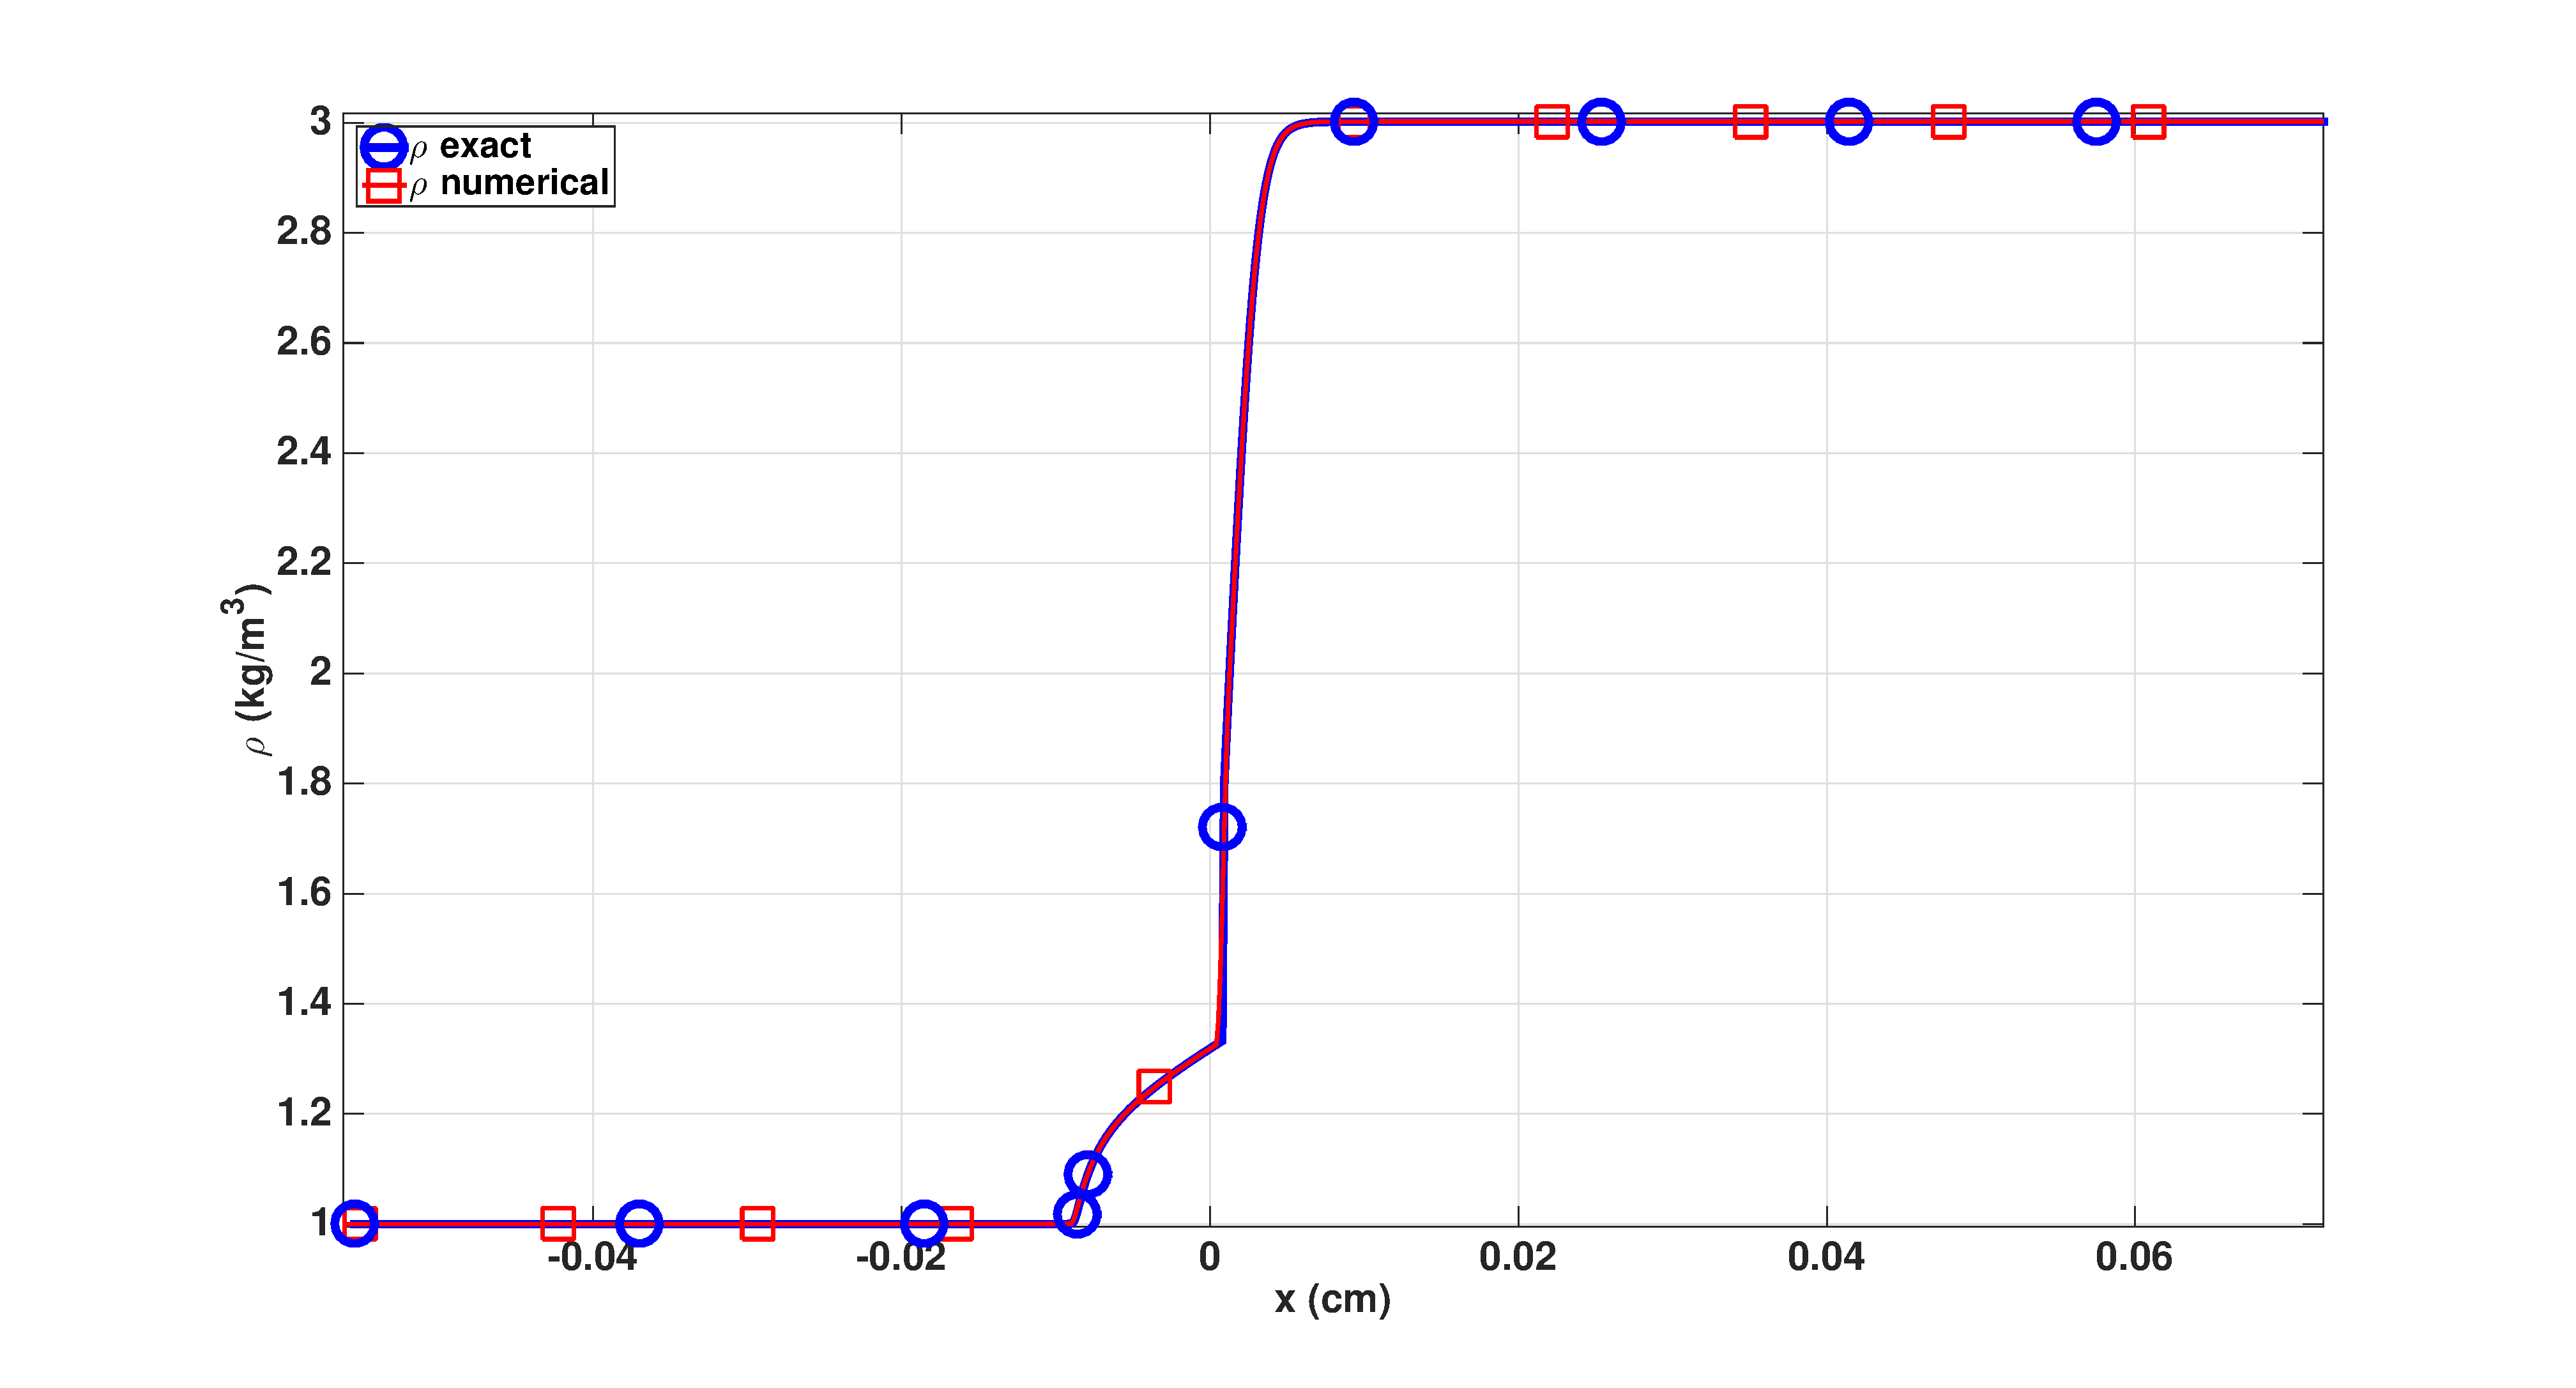
\includegraphics[width=\textwidth]{figures/dpt-xs/mach_3_nel_1000_density.eps}
    \caption{Steady-state material density for the Mach-3 shock test with temperature-dependent opacities.}\label{fig:mach-3-dpt-xs-dens}
\end{figure}
%
The density profile plotted in \fig{fig:mach-3-dpt-xs-dens} does not show any instability neither in the vicinity of the shock around $x = 0 \ cm$ nor in the abrupt change located at $x = -0.01 \ cm$. The shock is well resolved and the numerical and semi-analytical solutions overlap and are in excellent agreement.
%
\begin{figure}[H]
    \centering
    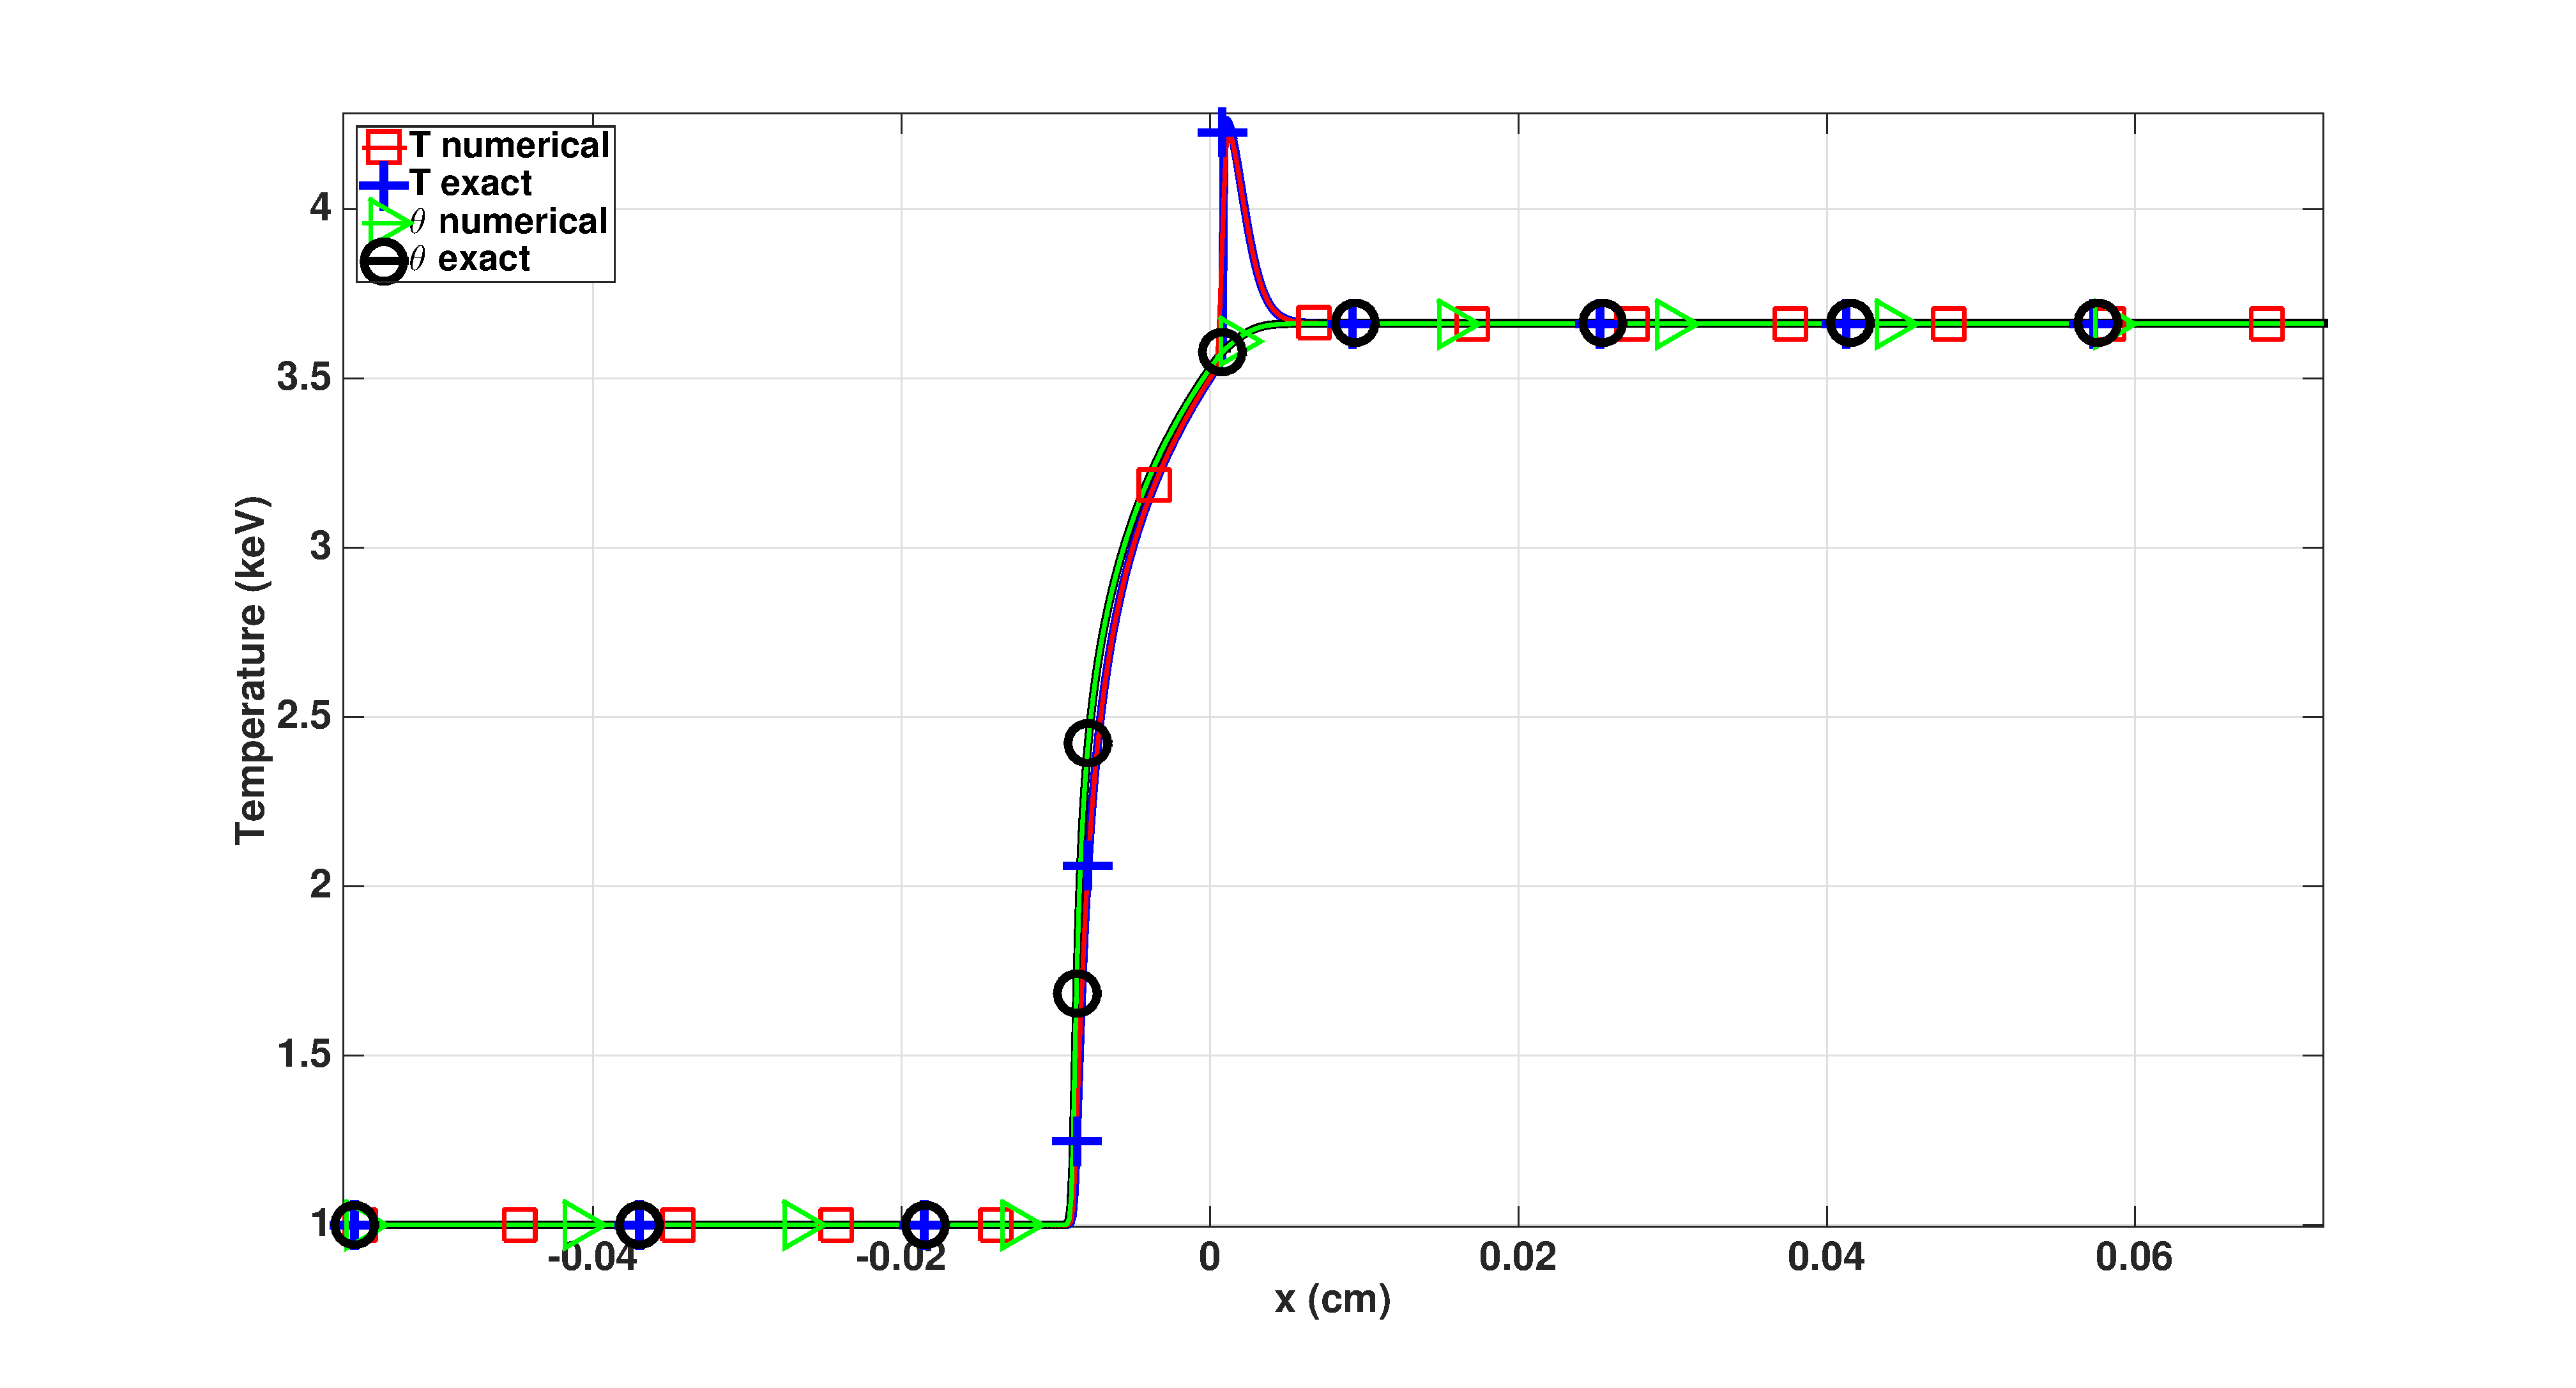
\includegraphics[width=\textwidth]{figures/dpt-xs/mach_3_nel_1000_temperature.eps}
    \caption{Steady-state material and radiation temperatures for the Mach-3 shock test with temperature-dependent opacities.}\label{fig:mach-3-dpt-xs-temp}
\end{figure}
%
In \fig{fig:mach-3-dpt-xs-temp}, the material and radiation temperatures do not show any instability either. The Zeldovich's pike in the material temperature profile is well resolved. The radiation temperature remains smooth as expected because of the diffusion term in the radiation equation. The numerical and semi-analytical solutions are in excellent agreement. 
%
\begin{figure}[H]
    \centering
    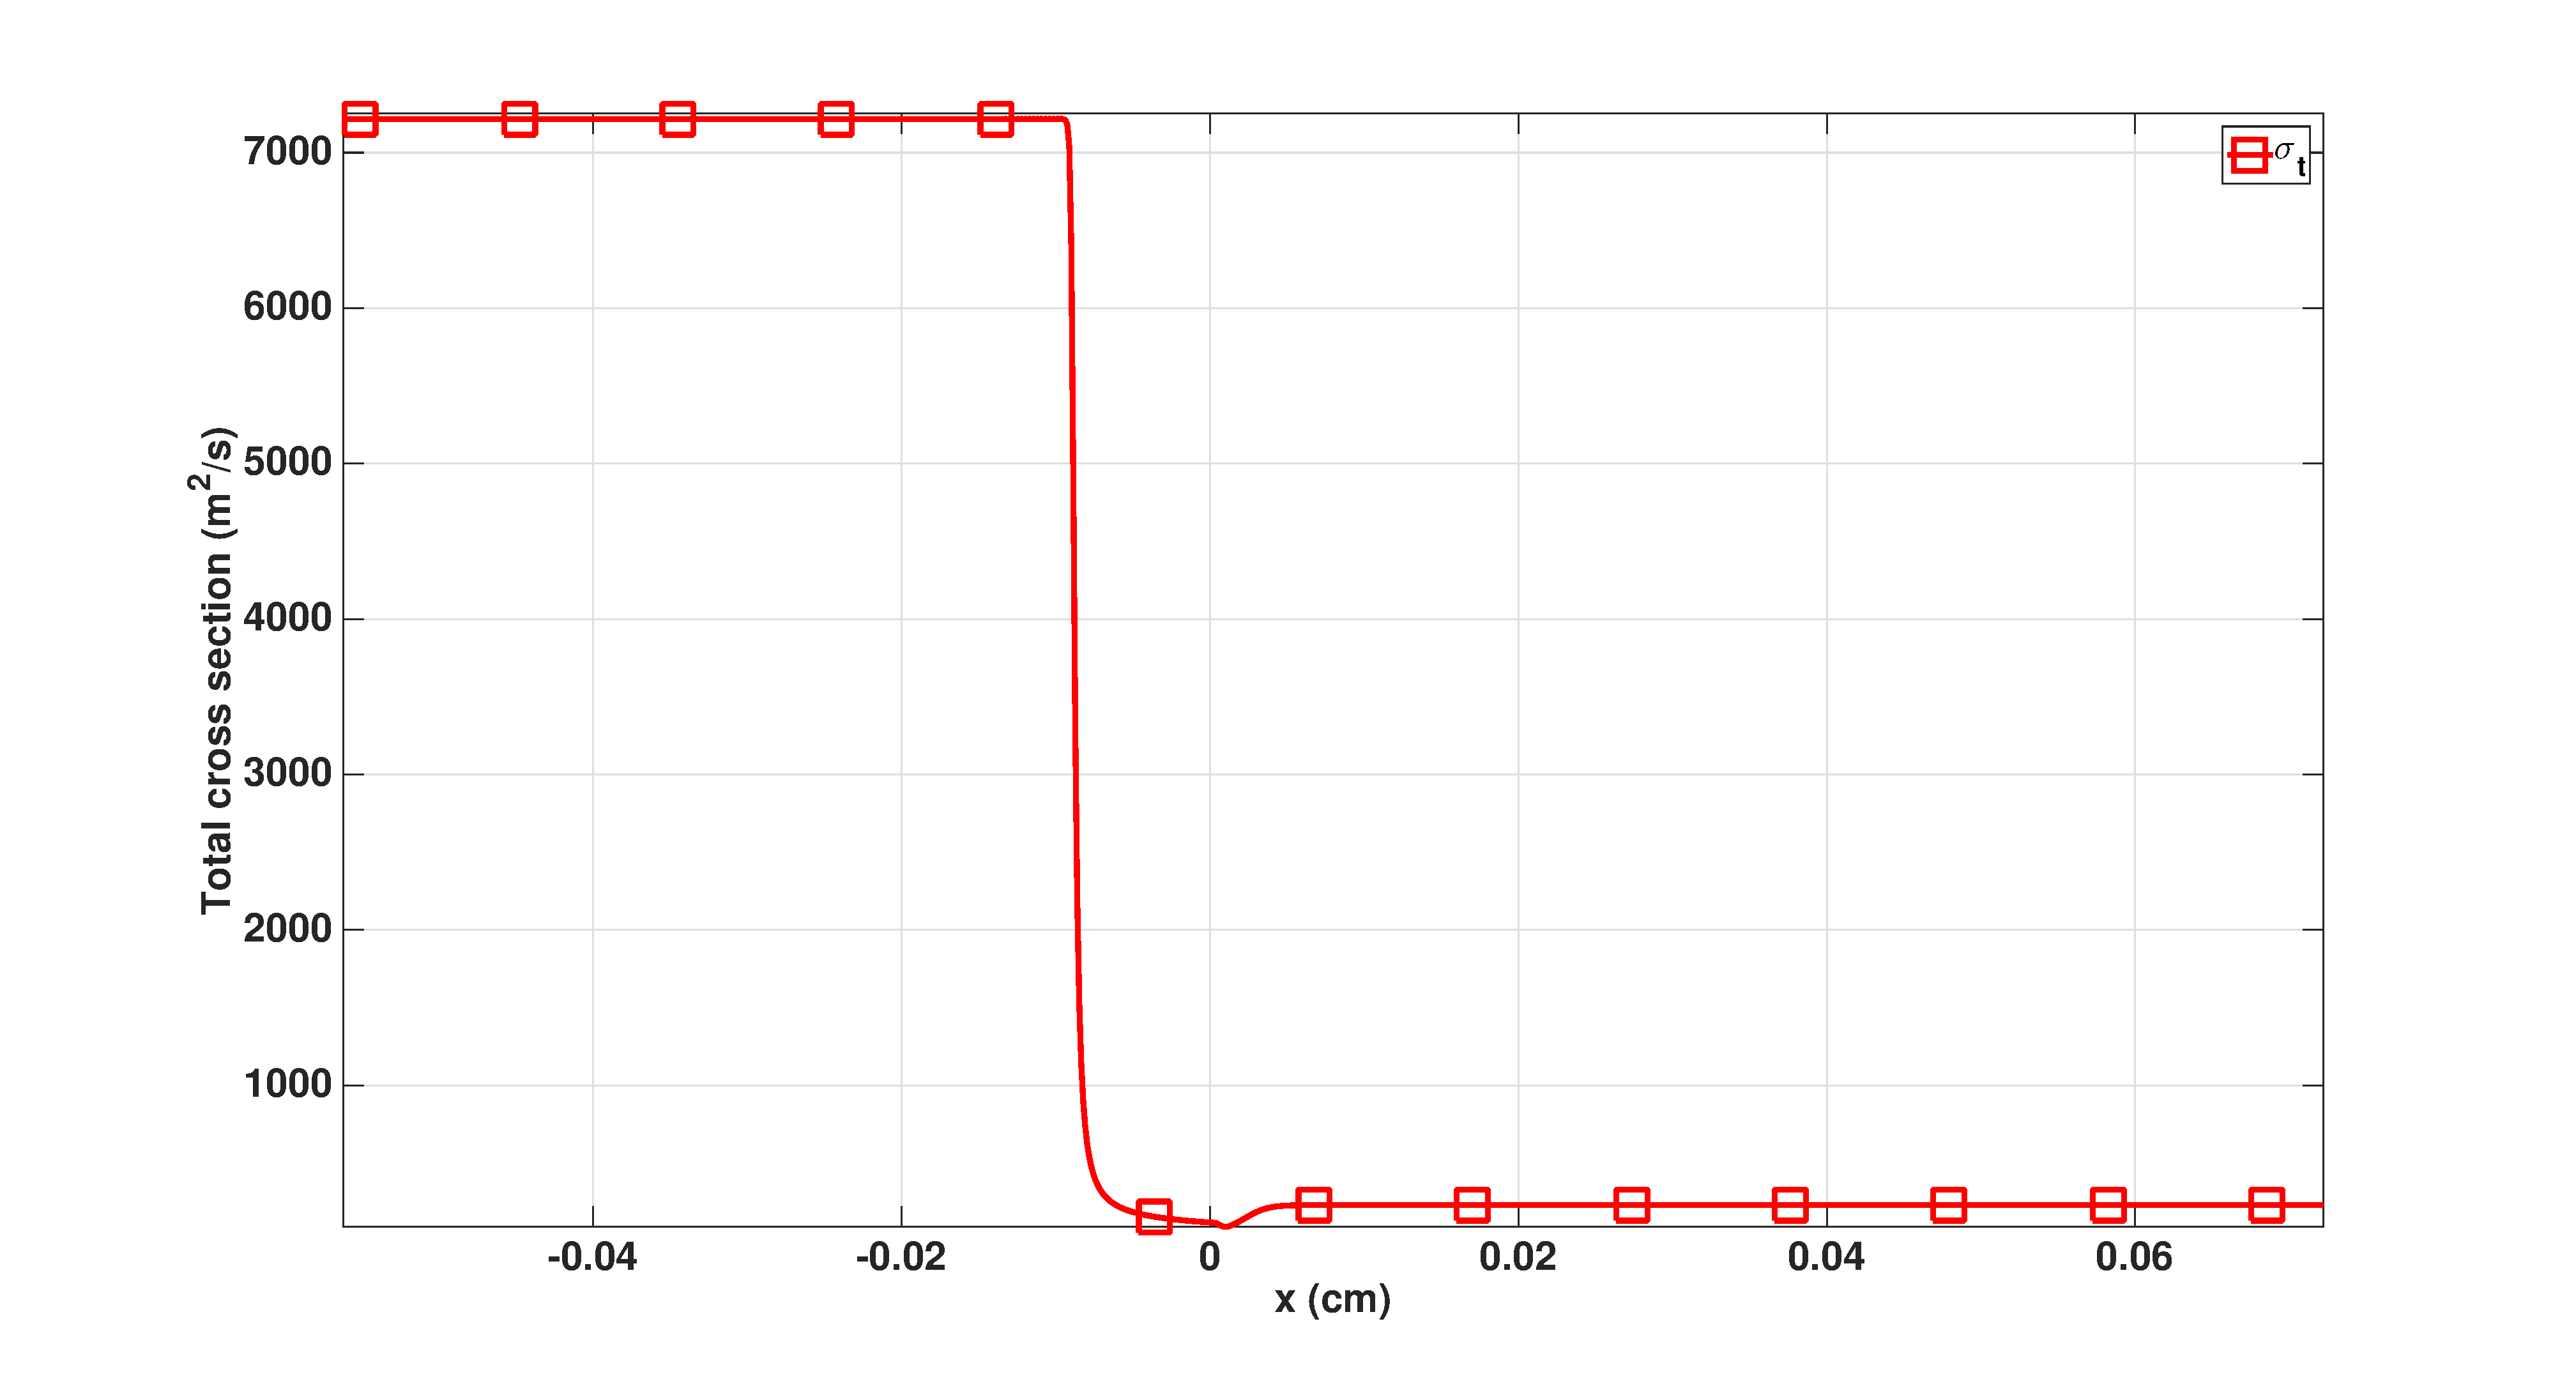
\includegraphics[width=\textwidth]{figures/dpt-xs/mach_3_nel_1000_total_cross_section.eps}
    \caption{Steady-state total opacity $\sigma_t$ for the Mach-3 shock test with temperature-dependent opacities.}\label{fig:mach-3-dpt-xs-xs}
\end{figure}
%
The numerical profile of the cross section is plotted in \fig{fig:mach-3-dpt-xs-xs} against the semi-analytical solution that was computed from the semi-analytical solutions of the material density and temperature. 
%
\end{document}